
El algoritmo de la Mochila entera o Mochila 0-1 o \textit{Knapsack}, hace uso de una tabla que suele llamarsele tabla dinámica, el llenado de la tabla es el algoritmo principal que se ejecuta para resolver la problemática de la mochila. El utilizar este método, en comparación con un implementación recursiva, elimina el traslape de subproblemas generados y por lo tanto disminuyendo el tiempo de ejecución.\\

La estructura de la tabla se conforma por tantas filas como objetos tengamos más una extra inicial, y se tendrán tantas columnas como peso máximo de la mochila se especifique, más 1 columna inicial con el valor de 0.\\

Las columnas ejemplifican el peso de la mochila partiendo desde un peso=0, hasta que se alcanza el peso máximo, y las filas corresponden a los pesos de los objetos según el orden que se tenga en el arreglo, más una fila primera que no corresponde a ningun peso y todos sus valores serán 0, esto es requisitado por el algoritmo para su correcto funcionamiento.\\

En el algoritmo utiliza las siguientes variables:\\
\begin{itemize}
    \item \textbf{P}: Peso máximo de la mochila
    \item \textbf{w}: Arreglo con los pesos de los objetos
    \item \textbf{b}: Arreglo con el valor de los objetos
    \item \textbf{c}: Variable auxiliar que indica el peso máximo correspondiente a la columna de la fila
    \item \textbf{g}: Tabla dinámica
\end{itemize}

El algoritmos para el llenado de esta tabla se muestra en la figura \ref{PseudocodigoKnapsack}:
\begin{figure}[h!]
    \centering
    \begin{verbatim}
        Entradas:w,b,P
        Salida:g
        
        for c=0 to c<=P do 
            g[0,c]=0
        for j=1 to j<=n do
            for c=1 to c<=P to
                if c<w[j-1]
                    g[j,c]=g[j-1,c]
                else
                    if g[j-1,c]>=g[j-1,c-w[j-1]]+b[j-1]
                        g[j,c]=g[j-1,c]
                    else
                        g[j,c]=g[j-1,c-w[j-1]]+b[j-1]
            
    \end{verbatim}
    \caption{Pseudocódigo del algoritmo que llena la tabla dinámica para el problema de la mochila entera}
    \label{PseudocodigoKnapsack}
\end{figure}


\newpage 

\subsection*{Interpretación de la tabla}
    Los valores en cada celda corresponden al valor máximo obtenible para el peso que representa la columna, para el conjunto de objetos que corresponden a la fila de la celda y las celdas anteriores, de forma que este valor es el óptimo para un peso máximo dado y un subconjunto de los objetos elegibles.\\
    
    Por esta razón el valor de la celda en la última columna(correspondiente al peso máximo ingresado de la mochila) en la última fila(correspondiente al peso del último objeto), será la solución con el beneficio máximo considerando todos los objetos elegibles para el peso total de la mochila restringido.\\

\section*{Complejidad}
    \subsection*{Análisis a \textit{priori}}    
        Para realizar el análisis a \textit{priori} nos referimos a la figura \ref{PseudocodigoKnapsack} para identificar la complejidad bloque a bloque:
        
        \begin{figure}[h!]
            \centering
            \begin{equation*}
                \left.
                    \begin{aligned}
                        \left.
                            \begin{aligned}
                                \text{for c=0 to c}<\text{=P do}\\
                                \text{  g[0,c] = 0 }
                            \end{aligned}
                        \right\}
                        \quad\Theta(P)\\
                    \left.
                        \begin{aligned}
                            \text{for j=1 to j}<\text{<=n do}\\
                            \left.
                                \begin{aligned}
                                    \text{for c=1 to c}<\text{=P to}\\
                                    \left.
                                        \begin{aligned}
                                            \left.
                                                \begin{aligned}
                                                    \text{if c}<\text{w[j-1]}\\
                                                    \text{g[j,c]=g[j-1,c]}\\
                                                    \text{else}
                                                \end{aligned}
                                            \right\}
                                            \quad\Theta(1)
                                            \\
                                            \left.
                                                \begin{aligned}
                                                    \text{if g[j-1,c]}>\text{=g[j-1,c-w[j-1]]+b[j-1]}\\
                                                    \text{g[j,c]=g[j-1,c]}\\
                                                    \text{else}\\
                                                    \text{g[j,c]=g[j-1,c-w[j-1]]+b[j-1]}
                                                \end{aligned}
                                            \right\}
                                            \quad\Theta(1)
                                        \end{aligned}
                                    \right\}
                                    \quad\Theta(1)
                                \end{aligned}
                            \right\}
                            \quad\Theta(P)
                        \end{aligned}
                    \right\}
                    \quad\Theta(n*P)
                    \end{aligned}
                \right\}
                \quad\Theta(n*P)+\Theta(P)=\Theta(n*P)
            \end{equation*}
            \caption{Complejidad por bloques de la función para la Mochila 0-1}
            \label{ComplejidadKnapsack}
        \end{figure}
        
    A diferencia de otros algoritmos que se han analizado vemos que la complejidad está en términos de 2 términos, previamente a este algoritmo se consideraba únicamente para el análisis un solo término el cual se considera fijo y a partir de este se consideraba el mejor y peor caso, en este algoritmo podríamos entonces considerar el peso máximo de la mochila(\textbf{P}) igual a 1 y tendríamos una complejidad lineal: $K(n,P) \in \Omega(n)$.\\
    
    Más esta premisa considera condiciones muy especiales en el que peso de la mochila es de solo 1 unidad, peso que tendría pocas aplicaciones reales, pero pensar en el valor mayor que pudiera tomar la \textbf{P} tampoco nos es factible, pues teoricamente este valor puede ser muy grande comparado con el número de objetos, no existe restricción para el valor de \textbf{P} más que sea mayor a 0 y pertenezca a los enteros naturales, dandole un límite de [1,$\infty$).\\
    
    Por estas consideraciones se concluye que la complejidad se encuentra en función de 2 términos(número de objetos seleccionables \textit{n}, y el peso máximo de la mochila \textit{P}) y corresponde al número de celdas que deben de ser llenadas para completar la tabla:\\
    \begin{equation*}
        K(n,P) \in \Theta(n*P)
    \end{equation*}
    
 \newpage
    
    \subsection*{Análisis a \textit{posteriori}}
        
        Se va a considerar para realizar el análisis a \textit{posteriori} 10 puntos en la gráfica, esto es 10 configuraciones de la mochila con pesos máximos diferentes para cada una y con la singularidad de que configuración tendrá un objeto más que la anterior empezando con 1 solo objeto el primer problema.\\
        
        La descripción de los puntos obtenidos el tipo de configuración utilizado se muestra en la figura \ref{PuntosKnapsack1}:
        \begin{figure}[h!]
            \centering
            \begin{tabular}{c c c}
                P1( 1 ,9 ) & \{ n=1 & P=6 \} \\
                P2( 2 ,25 ) & \{ n=2 & P=10 \} \\
                P3( 3 ,52 ) & \{ n=3 & P=15 \} \\
                P4( 4 ,29 ) & \{ n=4 & P=5 \} \\
                P5( 5 ,86 ) & \{ n=5 & P=15 \} \\
                P5( 6 ,61 ) & \{ n=6 & P=8 \} \\
                P7( 7 ,57 ) & \{ n=7 & P=6 \} \\
                P8( 8 ,201 ) & \{ n=8 & P=23 \} \\
                P8( 9 ,343 ) & \{ n=9 & P=36 \} \\
                P10( 10 ,91 ) & \{ n=10 & P=7 \} \\
            \end{tabular}
            \caption{Puntos obtenidos para la gráficación y la configuración de la mochila ingresada}
            \label{fig:my_label}
        \end{figure}
        
        La gráfica obtenida de estas configuraciones es la siguiente mostrada en la figura \ref{GraficaKnapsack1}:
        \begin{figure}[h!]
            \centering
            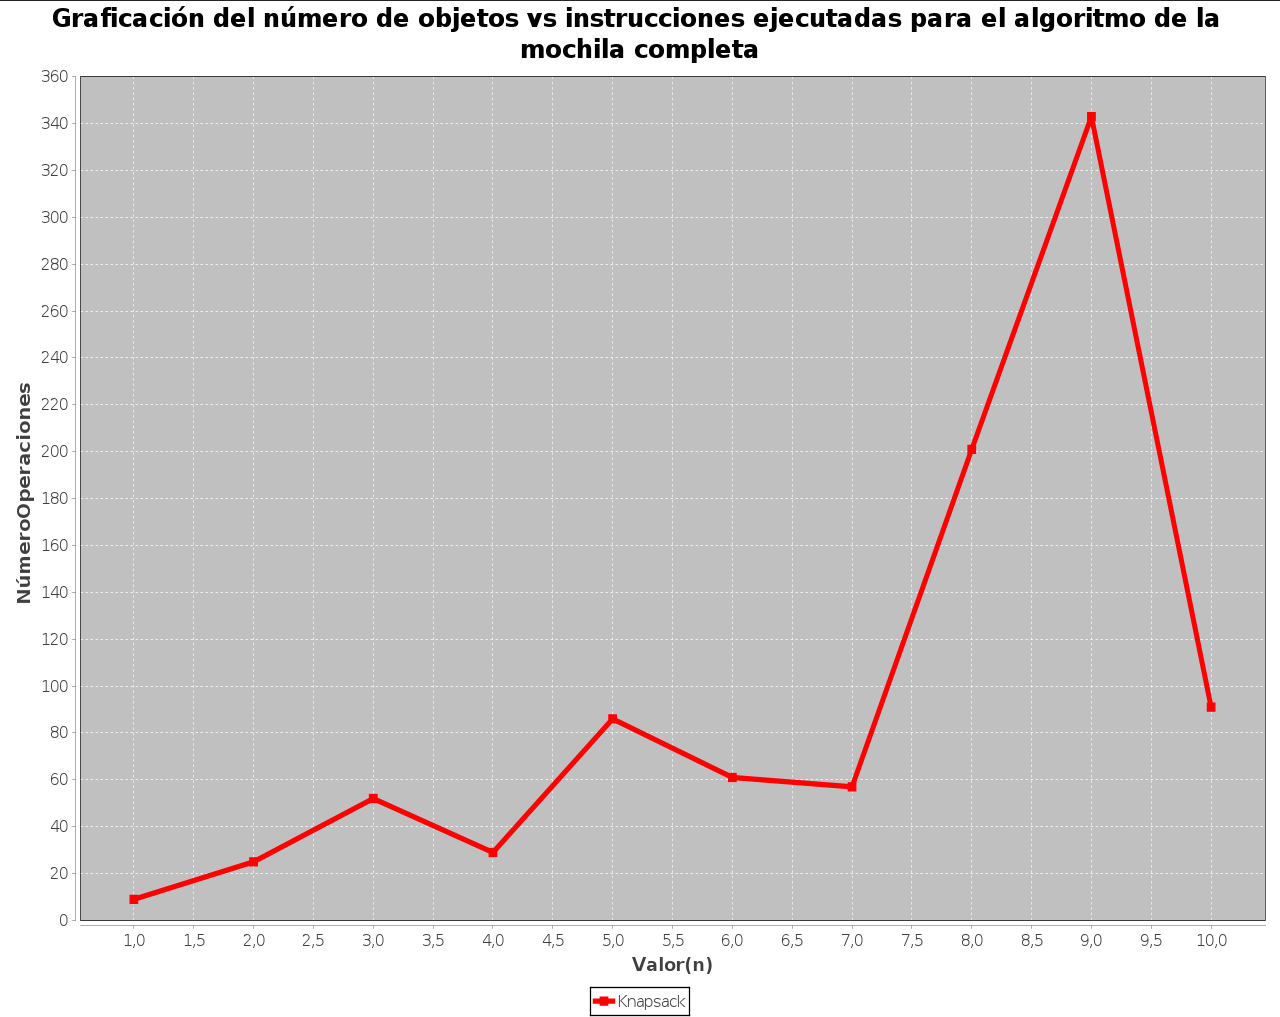
\includegraphics[width=15cm]{Knapsack/GraficaKnapsack1.png}
            \caption{Grafica obtenida de 10 problemas diferentes de la mochila entera con el número de objetos ascendentemente y un peso máximo de la mochila arbitrario para cada configuración}
            \label{GraficaKnapsack1}
        \end{figure}
        
        Se observa en la figura \ref{GraficaKnapsack1} una curva irregular que no nos aporta indicio alguno de la complejidad del algoritmo. Así pues intentamos mantener el orden ascendente del número de objetos pero consideraremos el valor de \textbf{P} igual a 10 en todas las configuraciones(figura \ref{GraficaKnapsack2} ):
        
        \begin{figure}[h!]
            \centering
            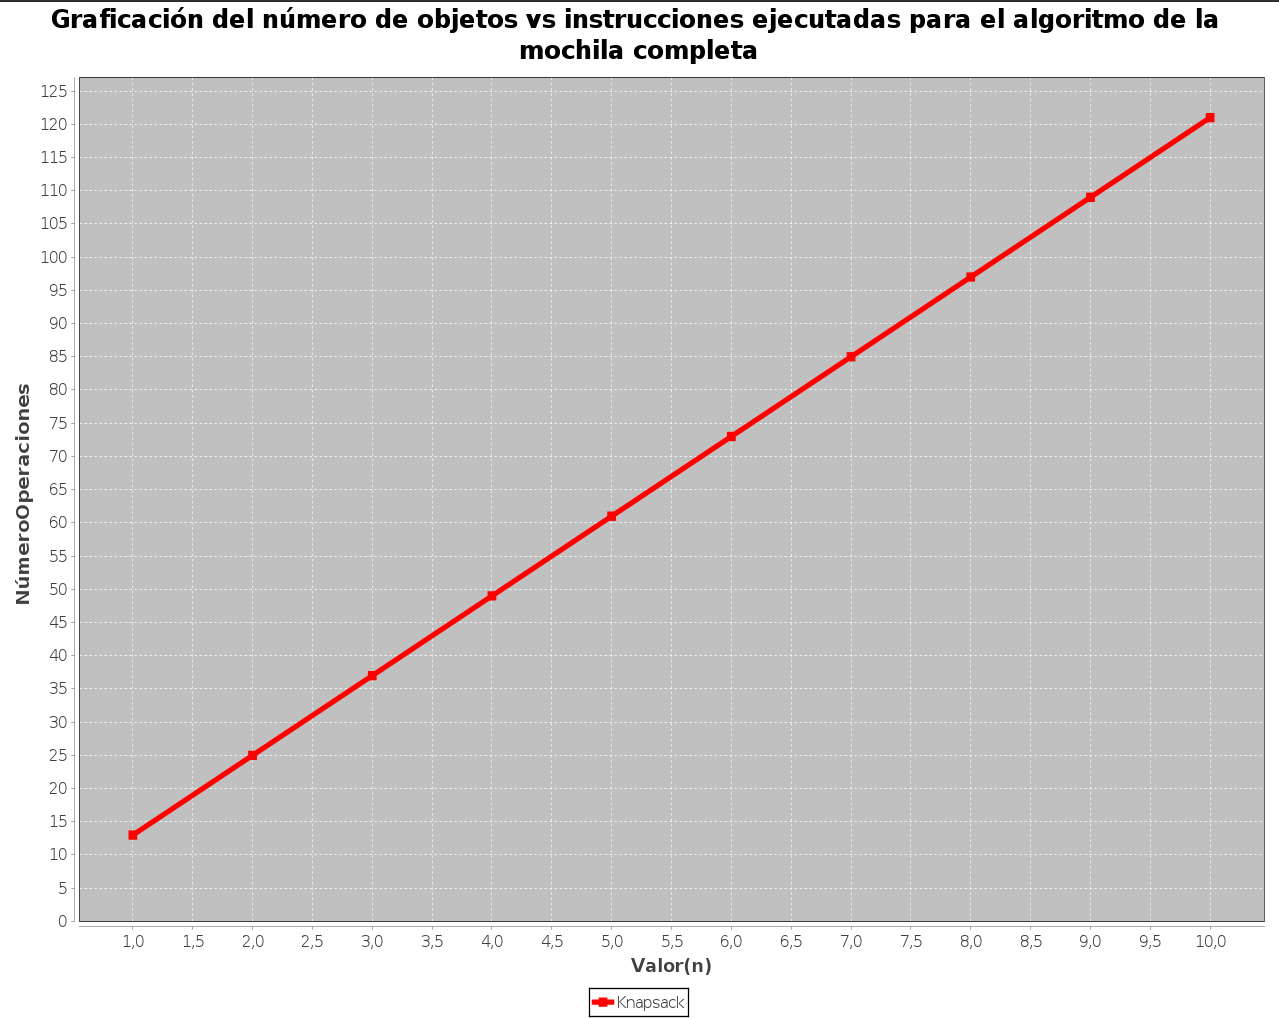
\includegraphics[width=15cm]{Knapsack/GraficaKnapsack2.png}
            \caption{Gráfica generada de 10 problemas diferentes para la mochila entera con un tamaño máximo para todas las mochilas igual}
            \label{GraficaKnapsack2}
        \end{figure}
        
        Y curiosamente para este tipo de configuración en la figura \ref{GraficaKnapsack2} se muestra una complejidad lineal, con una recta que se encuentra desplazada en el eje de las ordenadas, lo que nos sugeriría que existe o existen términos que multiplican a la \textbf{n} y/o que se suman como constante a la \textbf{n}, pudiendo ser el valor de \textbf{P} uno de estos términos.\\
        
        Por último para confirmar esta hipótesis se opta por asignar a cada configuración de mochilas $n=P$, generando la siguiente gráfica en la figura \ref{GraficaKnapsack3}:\\
        \begin{figure}[h!]
            \centering
            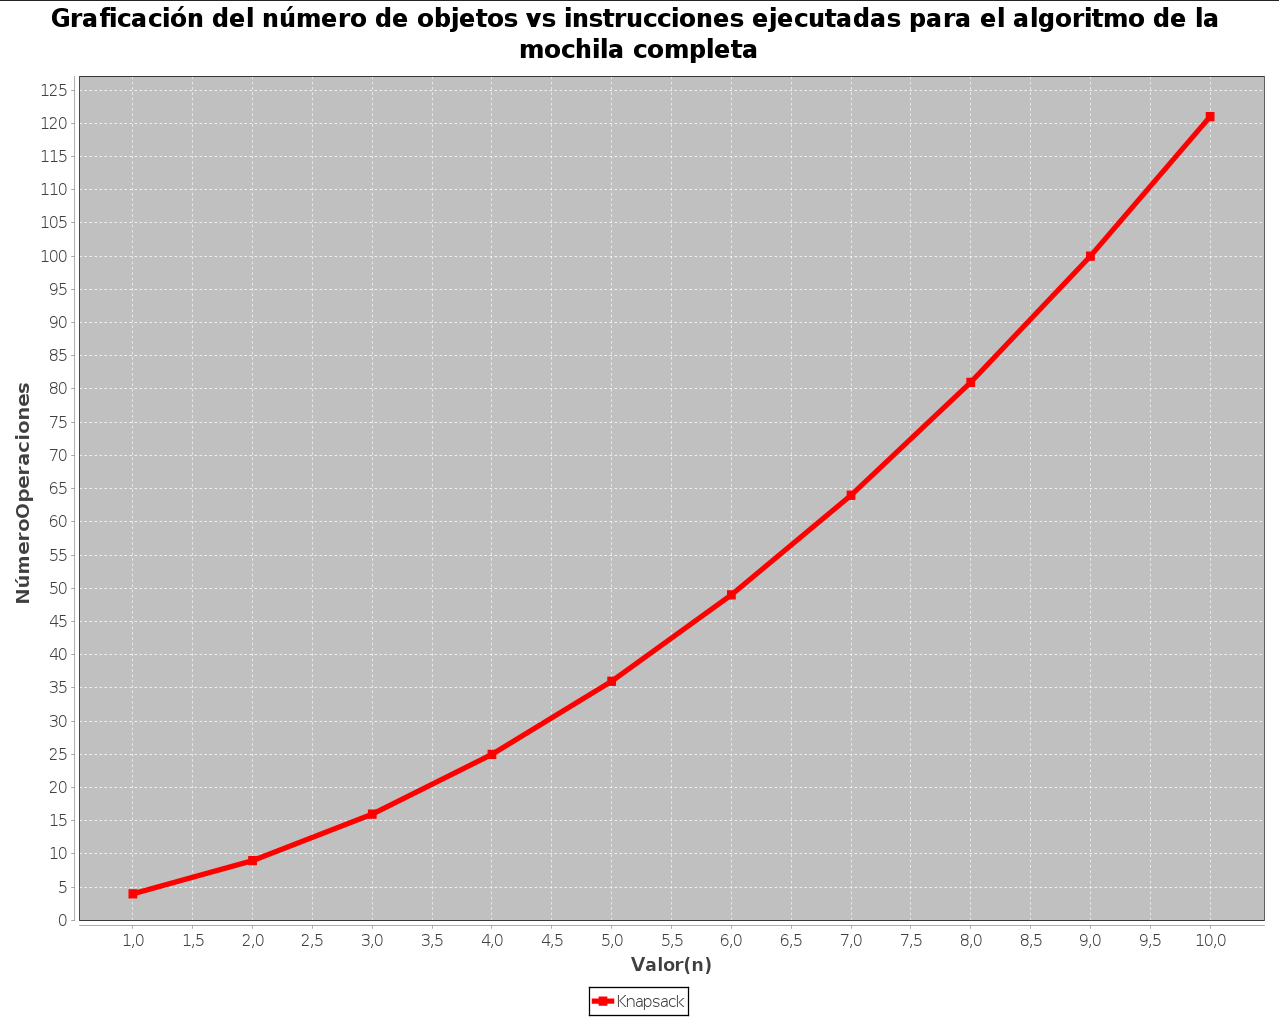
\includegraphics[width=15cm]{Knapsack/GraficaKnapsack3.png}
            \caption{Grafica obtenida para 10 problemas diferentes de la mochila entera donde el número de objetos es igual al peso máximo de la mochila \textbf{P}}
            \label{GraficaKnapsack3}
        \end{figure}
        La curva observada en la figura \ref{GraficaKnapsack3} nos confirma que el término \textbf{P} forma parte de un producto con el número de objetos seleccionables para obtener el comportamiento cuadrático mostrado, explicando así el desplazamiento de la curva en el eje de las ordenadas para la figura \ref{GraficaKnapsack2}, aunque siendo más estrictos para los puntos obtenidos es necesario agregar una constante que debe de pertenecer a las operaciones de asignación, entre otras, que utiliza el algoritmo.\\
        
        Con estas tres gráficas(\ref{GraficaKnapsack1},\ref{GraficaKnapsack2},\ref{GraficaKnapsack3}) afirmamos entonces que la complejidad del algoritmo para la mochila entera se encuentra en función del producto de \textbf{n} y \textbf{P}, quedándonos entonces:
        \begin{equation*}
            K(n,P) \in \Theta(n*P)
        \end{equation*}

\newpage

\section*{Función test}
    El método \textbf{test} funciona como un algoritmo de \textit{Backtracking}, de forma que va construyendo la solución a través de restricciones. Es necesaria esta función pues la construcción de la tabla nos va a asegurar el beneficio máximo para un peso máximo, pero no nos indica con que objetos construye este beneficio, cumpliendo esta necesidad el método \textbf{test}.\\
    
    Inicia su recorrido en la casilla para el beneficio máximo encontrado(celda en la última columna y última fila), y se desarrolla como una función espejo a la de la construcción de la misma tabla.\\
    
    Verifica si la celda en la misma columna pero de la fila anterior tiene un valor diferente, si no fuera el caso significaría que cuando se construyó la tabla, la solución óptima que no consideraba al objeto de la celda actual nos otorga un beneficio mayor a que se considerara este objeto, por lo tanto el valor de la fila anterior solamente es copiado en la fila actual; Esto implicaría en el método que se analiza que no fue construida la solución con este objeto y únicamente se realiza la siguiente iteración con la disminución en la unidad de la fila en la que se analiza la celda.\\
    
    En el caso contrario, donde el valor de la celda actual y el de la celda en la fila anterior sean diferentes, implica que en la elaboración de la tabla la consideración del beneficio del objeto actual nos otorga una solución mayor al de la obtenida para el mismo peso pero considerando unicamente los objetos anteriores;Esto permite considerar al método que el objeto correspondiente a esta fila participa en la suma para la obtención del beneficio máximo. Después entonces se agrega el objeto a los ingresados en la mochila, índice de las columnas disminuye tanto como el valor del peso del objeto correspondiente a la fila y se disminuye en la unidad el índice de la fila.\\
    
    Se itera esta condición hasta llegar a la primer celda, la cual siempre tendrá el valor 0, y es aquí cuando el algoritmo puede terminar su ejecución.\\
    
    La implementación de este algoritmo fue modificado para operar iterativamente, a diferencia del mostrado en el video de clase donde funciona de forma recursiva. El pseudocódigo entonces se muestra en la figura \ref{PseudocodigoTest}
    
    \begin{figure}[h!]
        \centering
        \begin{verbatim}
            Entrada:w
            Salida:m(Lista con los índices de los objetos que se deben ingresar en la mochila)
            
            fila=n+1
            columna=P+1
            while fila > 0 and columna > 0 do
                if g[fila,columna] != g[fila-1,columna]
                    m.push(fila-1)
                    columna = columna - w[fila-1]
                fila --
        \end{verbatim}
        \caption{Pseudocódigo de la implementación recursiva para el algoritmo \textbf{test}}
        \label{PseudocodigoTest}
    \end{figure}
    
    \subsection*{Pruebas funcionamiento}
        Para mostrar los resultados obtenidos de la función \textbf{test}, se van a considerar 2 problemas para la mochila entera:\\
        
        \textbf{Mochila con 5 objetos}\\
        
            Definimos una mochila con el peso máximo de \textbf{15} y la cual debemos de llenar con el máximo beneficio posible con 5 objetos dados(figura \ref{MochilaObjetos5}):
            
            \begin{figure}[h!]
                \centering
                    \begin{itemize}
                        \item Objeto 1 : w=12, b=4
                        \item Objeto 2 : w=2, b=2
                        \item Objeto 3 : w=1, b=1
                        \item Objeto 4 : w=4, b=10
                        \item Objeto 5 : w=1, b=2 
                    \end{itemize}
                \caption{Pesos y beneficio de cada uno de los 5 objetos seleccionables}
                \label{MochilaObjetos5}
            \end{figure}
            
            Se ingresan estos valores para que el algoritmo encuentre el beneficio máximo. A continuación en la figura \ref{ResultadosMochilaObjetos5} se muestrán los resultados del algoritmo:
            \begin{figure}[h!]
                \centering
                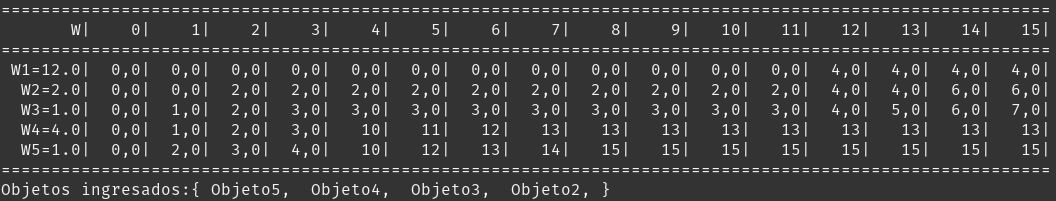
\includegraphics[width=\textwidth]{Knapsack/MochilaObjetos5.png}
                \caption{Resltados obtenidos: Tabla dinámica y el nombre de los elementos que deben de ser ingresados en la mochila para obtener el mayor beneficio}
                \label{ResultadosMochilaObjetos5}
            \end{figure}
            
            Según la última celda de la tabla dinámica, el beneficio máximo que podemos obtener es de \textbf{15}, y según el resultado del método \textbf{test} los objetos que nos otorgan este beneficio son los \textit{Objeto5,Objeto4,Objeto3} y el \textit{Objeto2}.\\
            
            Se realizamos la suma de los beneficios otorgados por estos objetos tenemos:
            $$ 2+1+10+2 = 15$$
            Concordando los resultados obtenidos por el método \textbf{test} con el beneficio máximo obtenible.
        
        \hfill \break
        \hfill \break
        
        \textbf{Mochila con 6 objetos}\\
        
            Ahora definimos una mochila con el peso máximo de \textbf{8} y esta mochila la debemos de llenar con el máximo beneficio posible con 6 objetos dados(figura \ref{MochilaObjetos6}):
            
            \begin{figure}[h!]
                \centering
                    \begin{itemize}
                        \item A : w=1, b=2
                        \item B : w=2, b=5
                        \item C : w=4, b=6
                        \item D : w=5, b=10
                        \item E : w=7, b=13 
                        \item F : w=9, b=16 
                    \end{itemize}
                \caption{Pesos y beneficio de cada uno de los 6 objetos seleccionables}
                \label{MochilaObjetos6}
            \end{figure}
            
            Se ingresan estos valores para que el algoritmo encuentre el beneficio máximo. A continuación en la figura \ref{ResultadosMochilaObjetos6} se muestrán los resultados del algoritmo:
            \begin{figure}[h!]
                \centering
                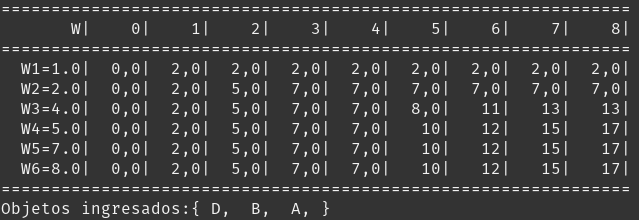
\includegraphics[width=\textwidth]{Knapsack/MochilaObjetos6.png}
                \caption{Resltados obtenidos: Tabla dinámica y el nombre de los elementos que deben de ser ingresados en la mochila para obtener el mayor beneficio}
                \label{ResultadosMochilaObjetos5}
            \end{figure}
            
            Según la última celda de la tabla dinámica, el beneficio máximo que podemos obtener es de \textbf{17}, y según el resultado del método \textbf{test} los objetos que nos otorgan este beneficio son \textit{D,B} y el objeto \textit{A}.\\
            
            Se realizamos la suma de los beneficios otorgados por estos objetos tenemos:
            $$ 10+5+2 = 17$$
            Concordando los resultados obtenidos por el método \textbf{test} con el beneficio máximo obtenible.
        
            